% +------------------------------------------------------------------------+
% | Reference manual page: Linear_cell_complex_constructors.tex
% +------------------------------------------------------------------------+
% | 04.02.2010   Guillaume Damiand
% | Package: Linear_cell_complex
% +------------------------------------------------------------------------+
\ccRefPageBegin
%%RefPage: end of header, begin of main body
% +------------------------------------------------------------------------+

%----------------------------------------------------------------------------
% \begin{ccRefFunction}{make_segment<LCC>}
% \ccInclude{Linear_cell_complex_constructors.h}\\

% \ccFunction{template <class LCC>
%   typename LCC::Dart_handle make_segment(LCC& lcc,
%   const typename LCC::Point& p0,  
%   const typename LCC::Point& p1);}
% {Creates an isolated segment in \ccc{lcc} (two darts linked by \betadeux{}) 
%   having \ccc{p0}, \ccc{p1} as geometry.
%    Returns an handle on the dart associated with \ccc{p0}.
%  \ccPrecond{\ccc{LCC::dimension}\mygeq{}2.}
% }
% %
% \def\LargFig{.3\textwidth}
%   \begin{ccTexOnly}
%     \begin{center}
%       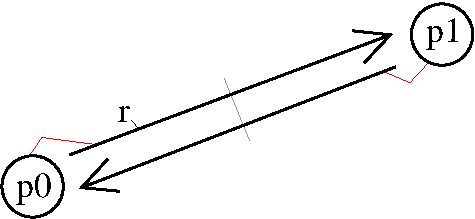
\includegraphics[width=\LargFig]{Linear_cell_complex_ref/fig/pdf/make_segment}
%     \end{center}
%   \end{ccTexOnly}
%   \begin{ccHtmlOnly}
%     <CENTER>
%     <A HREF="fig/png/make_segment.png">
%         <img src="../Linear_cell_complex_ref/fig/png/make_segment.png" alt=""></A>
%     </CENTER>
%     \end{ccHtmlOnly}
%     \centerline{Example of \ccc{r=make_segment(lcc,p0,p1)}.}
% \ccSeeAlso
% \ccRefIdfierPage{CGAL::make_triangle<LCC>}\\
% \ccRefIdfierPage{CGAL::make_quadrangle<LCC>}\\
% \ccRefIdfierPage{CGAL::make_rectangle<LCC>}\\
% %\ccRefIdfierPage{CGAL::make_rectangle2}\\
% %\ccRefIdfierPage{CGAL::make_square}\\
% \ccRefIdfierPage{CGAL::make_tetrahedron<LCC>}\\
% \ccRefIdfierPage{CGAL::make_hexahedron<LCC>}\\
% \ccRefIdfierPage{CGAL::make_iso_cuboid<LCC>}\\
% %\ccRefIdfierPage{CGAL::make_iso_cuboid2}\\
% %\ccRefIdfierPage{CGAL::make_cube}\\
% \end{ccRefFunction}
%----------------------------------------------------------------------------
% \begin{ccRefFunction}{make_triangle<LCC>}
% \ccInclude{Linear_cell_complex_constructors.h}\\

% \ccFunction{template <class LCC>
%   typename LCC::Dart_handle make_triangle(LCC& lcc,
%   const typename LCC::Point& p0,
%   const typename LCC::Point& p1,
%   const typename LCC::Point& p2);}  
% {Creates an isolated triangle in \ccc{lcc} having \ccc{p0}, \ccc{p1}, \ccc{p2} as geometry.
%    Returns an handle on the dart associated with \ccc{p0}.
%  \ccPrecond{\ccc{LCC::dimension}\mygeq{}1.}
% }
% %
% \def\LargFig{.3\textwidth}
%   \begin{ccTexOnly}
%     \begin{center}
%       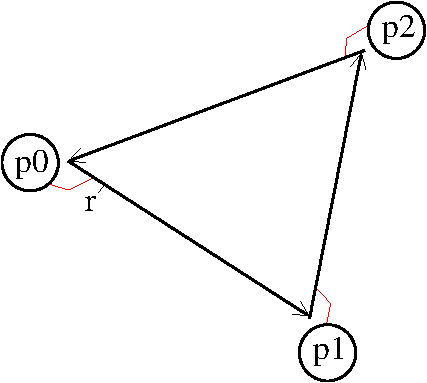
\includegraphics[width=\LargFig]{Linear_cell_complex_ref/fig/pdf/make_triangle}
%     \end{center}
%   \end{ccTexOnly}
%   \begin{ccHtmlOnly}
%     <CENTER>
%     <A HREF="fig/png/make_triangle.png">
%         <img src="../Linear_cell_complex_ref/fig/png/make_triangle.png" alt=""></A>
%     </CENTER>
%     \end{ccHtmlOnly}
%     \centerline{Example of \ccc{r=make_triangle(lcc,p0,p1,p2)}.}
% \ccSeeAlso
% \ccRefIdfierPage{CGAL::make_segment<LCC>}\\
% \ccRefIdfierPage{CGAL::make_quadrangle<LCC>}\\
% \ccRefIdfierPage{CGAL::make_rectangle<LCC>}\\
% %\ccRefIdfierPage{CGAL::make_rectangle2}\\
% %\ccRefIdfierPage{CGAL::make_square}\\
% \ccRefIdfierPage{CGAL::make_tetrahedron<LCC>}\\
% \ccRefIdfierPage{CGAL::make_hexahedron<LCC>}\\
% \ccRefIdfierPage{CGAL::make_iso_cuboid<LCC>}\\
% %\ccRefIdfierPage{CGAL::make_iso_cuboid2}\\
% %\ccRefIdfierPage{CGAL::make_cube}\\
% \end{ccRefFunction}
%----------------------------------------------------------------------------
% \begin{ccRefFunction}{make_quadrangle<LCC>}
% \ccInclude{Linear_cell_complex_constructors.h}\\

% \ccFunction{template <class LCC>
%   typename LCC::Dart_handle make_quadrangle(LCC& lcc,
%   const typename LCC::Point& p0,  
%   const typename LCC::Point& p1,  
%   const typename LCC::Point& p2,  
%   const typename LCC::Point& p3);}  
% {Creates an isolated quadrangle in \ccc{lcc}  having \ccc{p0} ,\ccc{p1}, 
%   \ccc{p2}, \ccc{p3} as geometry.
%    Returns an handle on the dart associated with \ccc{p0}.
%  \ccPrecond{\ccc{LCC::dimension}\mygeq{}1.}
% }
% %
% \def\LargFig{.3\textwidth}
%   \begin{ccTexOnly}
%     \begin{center}
%       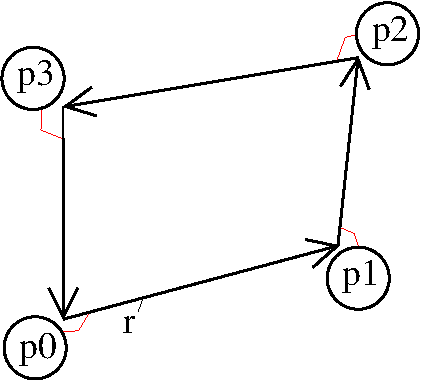
\includegraphics[width=\LargFig]{Linear_cell_complex_ref/fig/pdf/make_quadrilateral}
%     \end{center}
%   \end{ccTexOnly}
%   \begin{ccHtmlOnly}
%     <CENTER>
%     <A HREF="fig/png/make_quadrilateral.png">
%         <img src="../Linear_cell_complex_ref/fig/png/make_quadrilateral.png" alt=""></A>
%     </CENTER>
%     \end{ccHtmlOnly}
%     \centerline{Example of \ccc{r=make_quadrangle(lcc,p0,p1,p2,p3)}.}
% \ccSeeAlso
% \ccRefIdfierPage{CGAL::make_segment<LCC>}\\
% \ccRefIdfierPage{CGAL::make_triangle<LCC>}\\
% \ccRefIdfierPage{CGAL::make_rectangle<LCC>}\\
% %\ccRefIdfierPage{CGAL::make_rectangle2}\\
% %\ccRefIdfierPage{CGAL::make_square}\\
% \ccRefIdfierPage{CGAL::make_tetrahedron<LCC>}\\
% \ccRefIdfierPage{CGAL::make_hexahedron<LCC>}\\
% \ccRefIdfierPage{CGAL::make_iso_cuboid<LCC>}\\
% %\ccRefIdfierPage{CGAL::make_iso_cuboid2}\\
% %\ccRefIdfierPage{CGAL::make_cube}\\
% \end{ccRefFunction}
%----------------------------------------------------------------------------
% \begin{ccRefFunction}{make_rectangle<LCC>}
% \ccInclude{Linear_cell_complex_constructors.h}\\

% \ccFunction{template <class LCC>
%   typename LCC::Dart_handle make_rectangle(LCC& lcc,
%   const typename LCC::Iso_rectangle& ir);}
% {Creates an isolated rectangle in \ccc{lcc} having \ccc{ir} as geometry.
%    Returns an handle on the dart associated with \ccc{ir[0]}.
%  \ccPrecond{\ccc{LCC::dimension}\mygeq{}1 and \ccc{LCC::ambient_dimension}\mygeq{}2.}
% }

% \ccHeading{Requirements}
% \ccc{LCC::Traits} defines \ccc{Iso_rectangle_2} type.

%
% \ccSeeAlso
% \ccRefIdfierPage{CGAL::make_segment}\\
% \ccRefIdfierPage{CGAL::make_triangle}\\
% \ccRefIdfierPage{CGAL::make_quadrangle}\\
% %\ccRefIdfierPage{CGAL::make_square}\\
% \ccRefIdfierPage{CGAL::make_tetrahedron}\\
% \ccRefIdfierPage{CGAL::make_hexahedron}\\
% \ccRefIdfierPage{CGAL::make_iso_cuboid}\\
% \ccRefIdfierPage{CGAL::make_iso_cuboid2}\\
% %\ccRefIdfierPage{CGAL::make_cube}\\
% \end{ccRefFunction}
% %----------------------------------------------------------------------------
% \begin{ccRefFunction}{make_rectangle}
% \ccInclude{Linear_cell_complex_constructors.h}\\

% \ccFunction{template <class LCC>
%   typename LCC::Dart_handle make_rectangle(LCC& lcc,
%   const typename LCC::Point& p0,
%   const typename LCC::Point& p1);}
% {Creates an isolated rectangle in \ccc{lcc} having \ccc{p0} and \ccc{p1} as 
%   diagonal opposite points. Returns an handle on the dart associated with \ccc{p0}.
%  \ccPrecond{\ccc{LCC::dimension}\mygeq{}1 and \ccc{LCC::ambient_dimension}\mygeq{}2.}
% }

% \ccHeading{Requirements}
% \ccc{LCC::Traits} defines \ccc{Iso_rectangle_2} type.

%
% \def\LargFig{.3\textwidth}
%   \begin{ccTexOnly}
%     \begin{center}
%       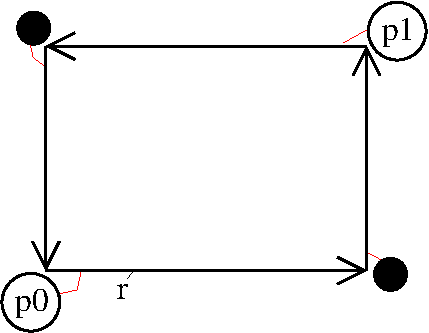
\includegraphics[width=\LargFig]{Linear_cell_complex_ref/fig/pdf/make_rectangle}
%     \end{center}
%   \end{ccTexOnly}
%   \begin{ccHtmlOnly}
%     <CENTER>
%     <A HREF="fig/png/make_rectangle.png">
%         <img src="../Linear_cell_complex_ref/fig/png/make_rectangle.png" alt=""></A>
%     </CENTER>
%     \end{ccHtmlOnly}
%     \centerline{Example of \ccc{r=make_rectangle(lcc,p0,p1)}.}

% \ccSeeAlso
% \ccRefIdfierPage{CGAL::make_segment<LCC>}\\
% \ccRefIdfierPage{CGAL::make_triangle<LCC>}\\
% \ccRefIdfierPage{CGAL::make_quadrangle<LCC>}\\
% %\ccRefIdfierPage{CGAL::make_rectangle2}\\
% %\ccRefIdfierPage{CGAL::make_square}\\
% \ccRefIdfierPage{CGAL::make_tetrahedron<LCC>}\\
% \ccRefIdfierPage{CGAL::make_hexahedron<LCC>}\\
% \ccRefIdfierPage{CGAL::make_iso_cuboid<LCC>}\\
% %\ccRefIdfierPage{CGAL::make_iso_cuboid2}\\
% %\ccRefIdfierPage{CGAL::make_cube}\\
% \end{ccRefFunction}
%----------------------------------------------------------------------------
% \begin{ccRefFunction}{make_square}
% \ccInclude{Linear_cell_complex_constructors.h}\\

% \ccFunction{template <class LCC>
%   typename LCC::Dart_handle make_square(LCC& lcc,
%   const typename LCC::Point& p,
%   typename LCC::FT l);}
% {Creates an isolated square in \ccc{lcc} having \ccc{p}  as based point, and \ccc{l} 
%   as size. Returns an handle on the dart associated with \ccc{p}.
%  \ccPrecond{\ccc{LCC::dimension}$\geq 1$ and \ccc{LCC::ambient_dimension}$\geq 2$.}
% }
% %
% \def\LargFig{.3\textwidth}
%   \begin{ccTexOnly}
%     \begin{center}
%       \includegraphics[width=\LargFig]{Linear_cell_complex_ref/fig/pdf/make_square}
%     \end{center}
%   \end{ccTexOnly}
%   \begin{ccHtmlOnly}
%     <CENTER>
%     <A HREF="fig/png/make_square.png">
%         <img src="../Linear_cell_complex_ref/fig/png/make_square.png" alt=""></A>
%     </CENTER>
%     \end{ccHtmlOnly}
%     \centerline{Example of \ccc{r=make_square(lcc,p,l)}.}
% \ccSeeAlso
% \ccRefIdfierPage{CGAL::make_segment}\\
% \ccRefIdfierPage{CGAL::make_triangle}\\
% \ccRefIdfierPage{CGAL::make_quadrangle}\\
% \ccRefIdfierPage{CGAL::make_rectangle}\\
% \ccRefIdfierPage{CGAL::make_tetrahedron}\\
% \ccRefIdfierPage{CGAL::make_hexahedron}\\
% \ccRefIdfierPage{CGAL::make_iso_cuboid}\\
% %\ccRefIdfierPage{CGAL::make_cube}\\
% \end{ccRefFunction}
%----------------------------------------------------------------------------
% \begin{ccRefFunction}{make_tetrahedron<LCC>}
% \ccInclude{Linear_cell_complex_constructors.h}\\

% \ccFunction{template <class LCC>
%   typename LCC::Dart_handle make_tetrahedron(LCC& lcc,
%   const typename LCC::Point& p0,
%   const typename LCC::Point& p1,
%   const typename LCC::Point& p2,
%   const typename LCC::Point& p3);}
% {Creates an isolated tetrahedron in \ccc{lcc} having \ccc{p0} ,\ccc{p1},\ccc{p2},\ccc{p3} as geometry.
%   Returns an handle on the dart associated with \ccc{p0} and
%   belonging to the 2-cell having \ccc{p0}, \ccc{p1}, \ccc{p2}
%   as coordinates.
%   \ccPrecond{\ccc{LCC::dimension}\mygeq{}2.}
% }
% %
% \def\LargFig{.3\textwidth}
%   \begin{ccTexOnly}
%     \begin{center}
%       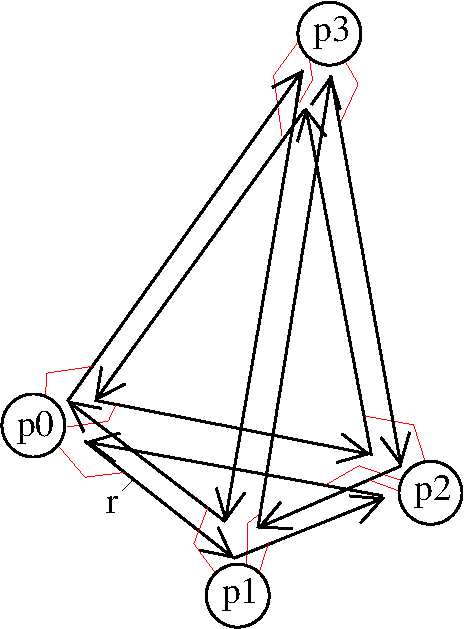
\includegraphics[width=\LargFig]{Linear_cell_complex_ref/fig/pdf/make_tetrahedron}
%     \end{center}
%   \end{ccTexOnly}
%   \begin{ccHtmlOnly}
%     <CENTER>
%     <A HREF="fig/png/make_tetrahedron.png">
%         <img src="../Linear_cell_complex_ref/fig/png/make_tetrahedron.png" alt=""></A>
%     </CENTER>
%     \end{ccHtmlOnly}
%     \centerline{Example of \ccc{r=make_tetrahedron(lcc,p0,p1,p2,p3)}.}
% \ccSeeAlso
% \ccRefIdfierPage{CGAL::make_segment<LCC>}\\
% \ccRefIdfierPage{CGAL::make_triangle<LCC>}\\
% \ccRefIdfierPage{CGAL::make_quadrangle<LCC>}\\
% \ccRefIdfierPage{CGAL::make_rectangle<LCC>}\\
% %\ccRefIdfierPage{CGAL::make_rectangle2}\\
% %\ccRefIdfierPage{CGAL::make_square}\\
% \ccRefIdfierPage{CGAL::make_hexahedron<LCC>}\\
% \ccRefIdfierPage{CGAL::make_iso_cuboid<LCC>}\\
% %\ccRefIdfierPage{CGAL::make_iso_cuboid2}\\
% %\ccRefIdfierPage{CGAL::make_cube}\\
% \end{ccRefFunction}
%----------------------------------------------------------------------------
% \begin{ccRefFunction}{make_hexahedron<LCC>}
% \ccInclude{Linear_cell_complex_constructors.h}\\

% \ccFunction{template <class LCC>
%   typename LCC::Dart_handle make_hexahedron(LCC& lcc,
%   const typename LCC::Point& p0,
%   const typename LCC::Point& p1,
%   const typename LCC::Point& p2,
%   const typename LCC::Point& p3,
%   const typename LCC::Point& p4,
%   const typename LCC::Point& p5,
%   const typename LCC::Point& p6,
%   const typename LCC::Point& p7);}
% {Creates an isolated hexahedron in \ccc{lcc} having \ccc{p0}, \ccc{p1},
% \ccc{p2}, \ccc{p3}, \ccc{p4}, \ccc{p5}, \ccc{p6}, \ccc{p7} as geometry.
%   Returns an handle on the dart associated with \ccc{p0} and
%   belonging to the 2-cell having \ccc{p0}, \ccc{p5}, \ccc{p6}, \ccc{p1}
%   as coordinates.
%   \ccPrecond{\ccc{LCC::dimension}\mygeq{}2.}
% }
% \def\LargFig{.4\textwidth}
%   \begin{ccTexOnly}
%     \begin{center}
%       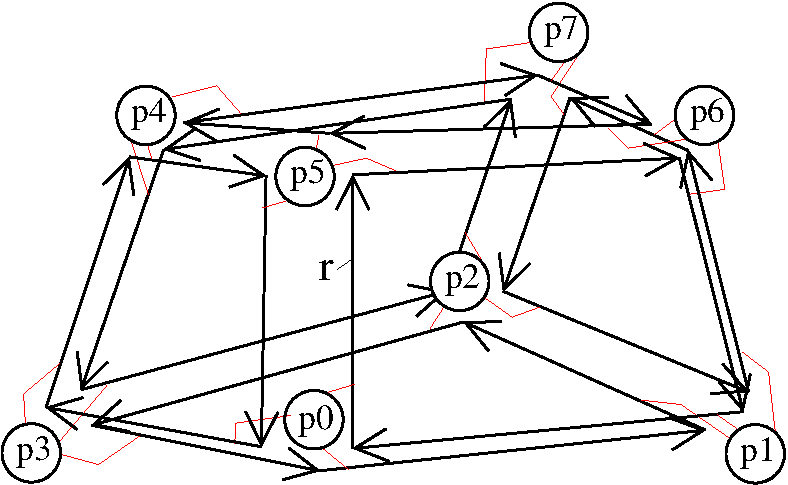
\includegraphics[width=\LargFig]{Linear_cell_complex_ref/fig/pdf/make_hexahedron}
%     \end{center}
%   \end{ccTexOnly}
%   \begin{ccHtmlOnly}
%     <CENTER>
%     <A HREF="fig/png/make_hexahedron.png">
%         <img src="../Linear_cell_complex_ref/fig/png/make_hexahedron.png" alt=""></A>
%     </CENTER>
%     \end{ccHtmlOnly}
%     \centerline{Example of \ccc{r=make_hexahedron(lcc,p0,p1,p2,p3,p4,p5,p6,p7)}.}
% \ccSeeAlso
% \ccRefIdfierPage{CGAL::make_segment<LCC>}\\
% \ccRefIdfierPage{CGAL::make_triangle<LCC>}\\
% \ccRefIdfierPage{CGAL::make_quadrangle<LCC>}\\
% \ccRefIdfierPage{CGAL::make_rectangle<LCC>}\\
% %\ccRefIdfierPage{CGAL::make_rectangle2}\\
% %\ccRefIdfierPage{CGAL::make_square}\\
% \ccRefIdfierPage{CGAL::make_tetrahedron<LCC>}\\
% \ccRefIdfierPage{CGAL::make_iso_cuboid<LCC>}\\
% %\ccRefIdfierPage{CGAL::make_iso_cuboid2}\\
% %\ccRefIdfierPage{CGAL::make_cube}\\
% \end{ccRefFunction}
%----------------------------------------------------------------------------
% \begin{ccRefFunction}{make_iso_cuboid<LCC>}
% \ccInclude{Linear_cell_complex_constructors.h}\\

% \ccFunction{template <class LCC>
%   typename LCC::Dart_handle make_iso_cuboid(LCC& lcc,
%   const typename LCC::Iso_cuboid& ic);}
% {Creates an isolated cuboid in \ccc{lcc} having points in \ccc{ic} as points.
%   Returns an handle on the dart associated with \ccc{ic[0]},
%   and belonging to the 2-cell having
%   \ccc{ic[0]},\ccc{ic[5]}, \ccc{ic[6]},\ccc{ic[1]} as coordinates.
%   \ccPrecond{\ccc{LCC::dimension}\mygeq{}2 and \ccc{LCC::ambient_dimension}\mygeq{}3.}
% }

% \ccHeading{Requirements}
% \ccc{LCC} defines \ccc{Iso_cuboid} type.

%
% \def\LargFig{.4\textwidth}
%   \begin{ccTexOnly}
%     \begin{center}
%       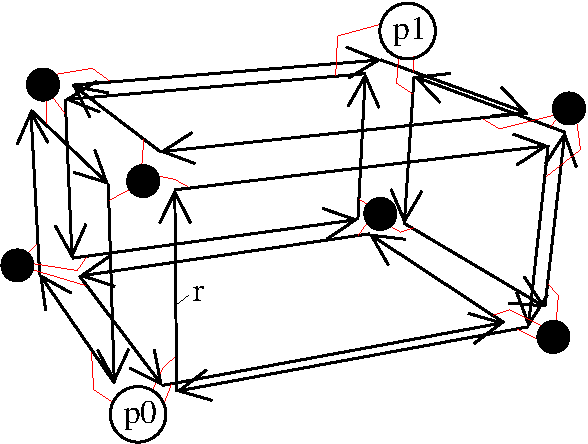
\includegraphics[width=\LargFig]{Linear_cell_complex_ref/fig/pdf/make_cuboid}
%     \end{center}
%   \end{ccTexOnly}
%   \begin{ccHtmlOnly}
%     <CENTER>
%     <A HREF="fig/png/make_cuboid.png">
%         <img src="../Linear_cell_complex_ref/fig/png/make_cuboid.png" alt=""></A>
%     </CENTER>
%     \end{ccHtmlOnly}
%     \centerline{Example of \ccc{r=make_iso_cuboid(lcc,ic)}.}
% \ccSeeAlso
% \ccRefIdfierPage{CGAL::make_segment}\\
% \ccRefIdfierPage{CGAL::make_triangle}\\
% \ccRefIdfierPage{CGAL::make_quadrangle}\\
% \ccRefIdfierPage{CGAL::make_rectangle}\\
% %\ccRefIdfierPage{CGAL::make_rectangle2}\\
% %\ccRefIdfierPage{CGAL::make_square}\\
% \ccRefIdfierPage{CGAL::make_tetrahedron}\\
% \ccRefIdfierPage{CGAL::make_hexahedron}\\
% \ccRefIdfierPage{CGAL::make_iso_cuboid}\\
% %\ccRefIdfierPage{CGAL::make_cube}\\
% \end{ccRefFunction}
% %%----------------------------------------------------------------------------
% \begin{ccRefFunction}{make_iso_cuboid}
% \ccInclude{Linear_cell_complex_constructors.h}\\

% \ccFunction{template <class LCC>
%   typename LCC::Dart_handle make_iso_cuboid(LCC& lcc,
%   const typename LCC::Point& p0,
%   const typename LCC::Point& p1);}
%   {Creates an isolated cuboid in \ccc{lcc} given having \ccc{p0} and
%     \ccc{p1} as diagonal opposite points. We denote by \ccc{ic} the
%     \ccc{Iso_cuboid_3} build from \ccc{p0} and \ccc{p1}.  
%       Returns an handle on the dart associated with \ccc{ic[0]},
%       and belonging to the 2-cell having
%       \ccc{ic[0]},\ccc{ic[5]}, \ccc{ic[6]},\ccc{ic[1]} as coordinates.
%       \ccPrecond{\ccc{LCC::dimension}\mygeq{}2 and \ccc{LCC::ambient_dimension}\mygeq{}3.}
% }

% \ccHeading{Requirements}
% \ccc{LCC} defines \ccc{Iso_cuboid} type.

%
% \def\LargFig{.4\textwidth}
%   \begin{ccTexOnly}
%     \begin{center}
%       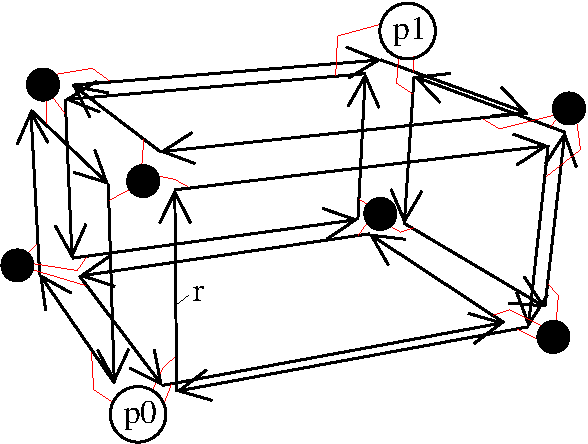
\includegraphics[width=\LargFig]{Linear_cell_complex_ref/fig/pdf/make_cuboid}
%     \end{center}
%   \end{ccTexOnly}
%   \begin{ccHtmlOnly}
%     <CENTER>
%     <A HREF="fig/png/make_cuboid.png">
%         <img src="../Linear_cell_complex_ref/fig/png/make_cuboid.png" alt=""></A>
%     </CENTER>
%     \end{ccHtmlOnly}
%     \centerline{Example of \ccc{r=make_iso_cuboid(lcc,p0,p1)}.}

% \ccSeeAlso
% \ccRefIdfierPage{CGAL::make_segment<LCC>}\\
% \ccRefIdfierPage{CGAL::make_triangle<LCC>}\\
% \ccRefIdfierPage{CGAL::make_quadrangle<LCC>}\\
% \ccRefIdfierPage{CGAL::make_rectangle<LCC>}\\
% %\ccRefIdfierPage{CGAL::make_rectangle2}\\
% %\ccRefIdfierPage{CGAL::make_square}\\
% \ccRefIdfierPage{CGAL::make_tetrahedron<LCC>}\\
% \ccRefIdfierPage{CGAL::make_hexahedron<LCC>}\\
% %\ccRefIdfierPage{CGAL::make_iso_cuboid2}\\
% %\ccRefIdfierPage{CGAL::make_cube}\\
% \end{ccRefFunction}
%----------------------------------------------------------------------------
% \begin{ccRefFunction}{make_cube}
% \ccInclude{Linear_cell_complex_constructors.h}\\

% \ccFunction{typename LCC::Dart_handle make_cube(LCC& lcc,
%                                     const typename LCC::Point& p,
%                                     typename LCC::FT l);}
% {Creates an isolated cube in \ccc{lcc} having \ccc{p} as based point, and
%   \ccc{l} as size.
%   Returns an handle on the dart associated with \ccc{p},
%   and belonging to the 2-cell having
%   \ccc{p},\ccc{p}+(0,0,\ccc{l}), \ccc{p}+(\ccc{l},0,\ccc{l}), \ccc{a}+(\ccc{l},0,0). 
%   as coordinates.
%   \ccPrecond{\ccc{LCC::dimension}$\geq 2$ and \ccc{LCC::ambient_dimension}$\geq 3$.}
% }
% %
% \def\LargFig{.3\textwidth}
%   \begin{ccTexOnly}
%     \begin{center}
%       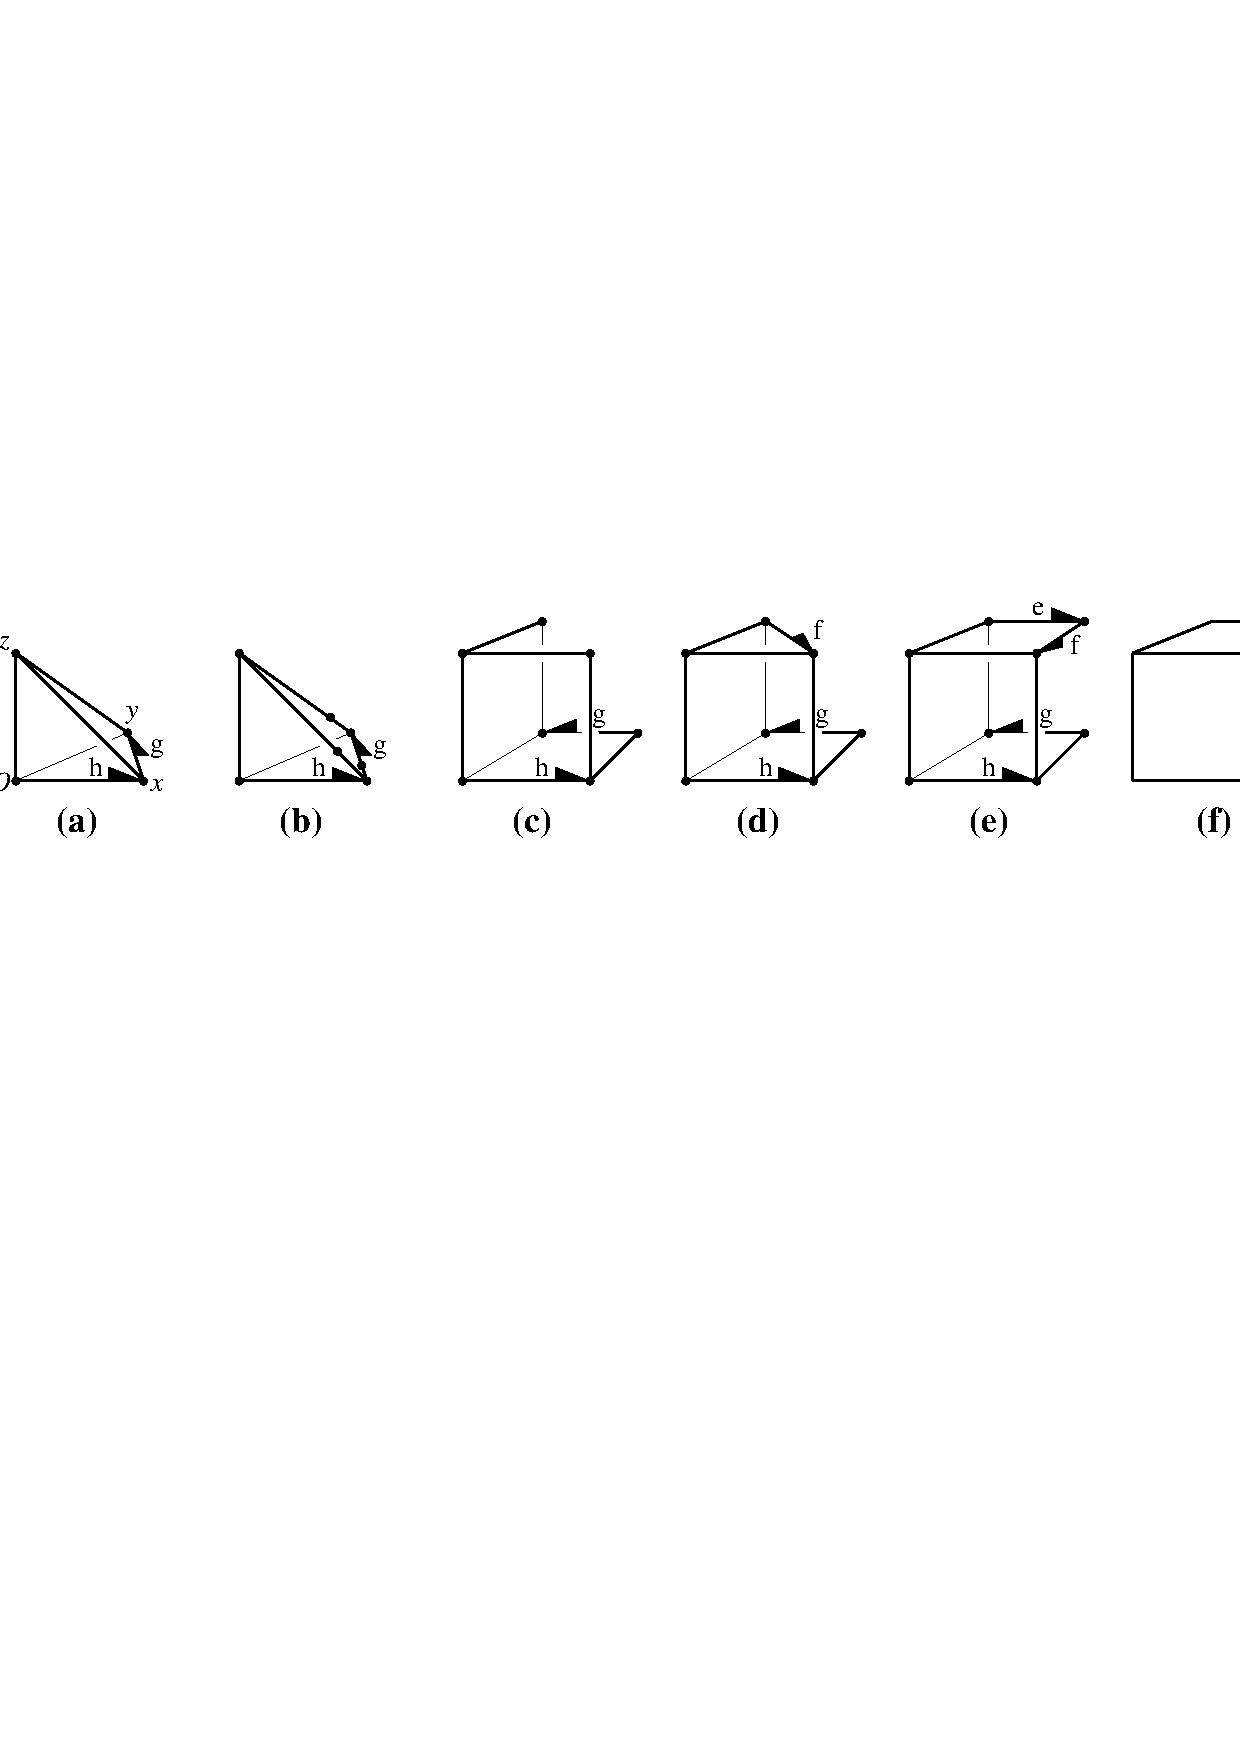
\includegraphics[width=\LargFig]{Linear_cell_complex_ref/fig/pdf/make_cube}
%     \end{center}
%   \end{ccTexOnly}
%   \begin{ccHtmlOnly}
%     <CENTER>
%     <A HREF="fig/png/make_cube.png">
%         <img src="../Linear_cell_complex_ref/fig/png/make_cube.png" alt=""></A>
%     </CENTER>
%     \end{ccHtmlOnly}
%     \centerline{Example of \ccc{r=make_cube(lcc,p,l)}.}
% \ccSeeAlso
% \ccRefIdfierPage{CGAL::make_segment}\\
% \ccRefIdfierPage{CGAL::make_triangle}\\
% \ccRefIdfierPage{CGAL::make_quadrangle}\\
% \ccRefIdfierPage{CGAL::make_rectangle}\\
% %\ccRefIdfierPage{CGAL::make_square}\\
% \ccRefIdfierPage{CGAL::make_tetrahedron}\\
% \ccRefIdfierPage{CGAL::make_hexahedron}\\
% \ccRefIdfierPage{CGAL::make_iso_cuboid}\\
% \end{ccRefFunction}
%----------------------------------------------------------------------------
\begin{ccRefFunction}{import_from_plane_graph<LCC>}
\ccInclude{Linear_cell_complex_constructors.h}\\

\ccFunction{template<class LCC>
  typename LCC::Dart_handle import_from_plane_graph(LCC& lcc,
  std::istream& ais);}
{Converts an embedded plane graph read from \ccc{ais} into \ccc{lcc}. 
  Objects are added in \ccc{lcc}, existing objects are not modified.
  Returns a dart created during the import.
  \ccPrecond{\ccc{LCC::dimension}\mygeq{}2 and \ccc{LCC::ambient_dimension}==2.}
}

\ccHeading{File format}
The file format must be the following: 
\begin{itemize}
\item first line: \verb|nbvertices nbedges|;
\item \verb|nbvertices| lines: \verb|x y| the coordinates of the \myith{} vertex;
\item \verb|nbedges| lines: \verb|i j| the index of the two vertices of the edge (first vertex
being 0).
\end{itemize}

Here a small example:
\begin{verbatim}
5 6

1.0 3.0
0.0 2.0
2.0 2.0
0.0 0.0
2.0 0.0

0 1
0 2
1 2
1 3
2 4
3 4
\end{verbatim}
%
\def\LargFig{.6\textwidth}
  \begin{ccTexOnly}
    \begin{center}
      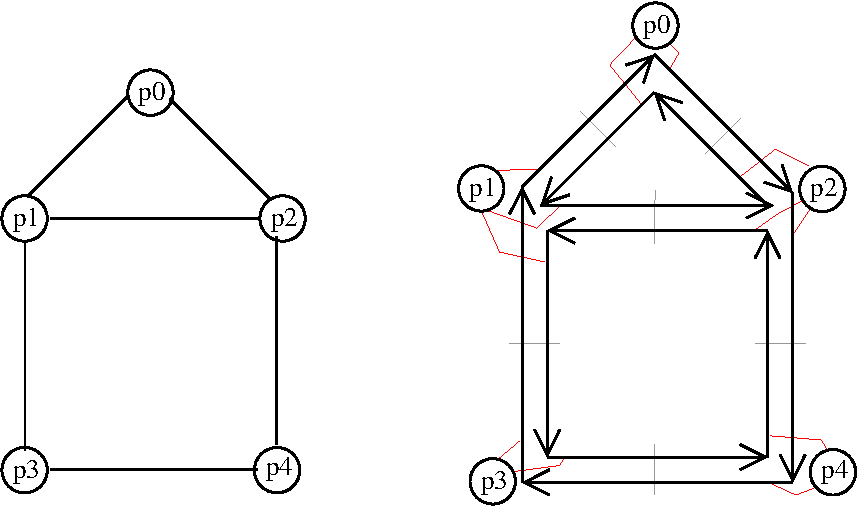
\includegraphics[width=\LargFig]{Linear_cell_complex_ref/fig/pdf/import_graph}
    \end{center}
  \end{ccTexOnly}
  \begin{ccHtmlOnly}
    <CENTER>
    <A HREF="fig/png/import_graph.png">
        <img src="../Linear_cell_complex_ref/fig/png/import_graph.png" alt=""></A>
    </CENTER>
    \end{ccHtmlOnly}
    \begin{center}
      Example of \ccc{import_graph} reading the above file as istream. \\
      \textbf{Left}: A planar graph embedded in the plane with 
      \emph{P0}=(1.0,3.0), \emph{P1}=(0.0,2.0), \emph{P2}=(2.0,2.0), \emph{P3}=(0.0,0.0), \emph{P4}=(2.0,0.0).
      \textbf{Right}: the 2D linear cell complex reconstructed.
      \end{center}
\ccSeeAlso
\ccRefIdfierPage{CGAL::import_from_triangulation_3<LCC,Triangulation>}\\
\ccRefIdfierPage{CGAL::import_from_polyhedron<LCC,Polyhedron>}\\
\end{ccRefFunction}
%----------------------------------------------------------------------------
\begin{ccRefFunction}{import_from_triangulation_3<LCC,Triangulation>}
\ccInclude{Linear_cell_complex_constructors.h}\\

\ccFunction{template <class LCC,class Triangulation_>
   typename LCC::Dart_handle import_from_triangulation_3(LCC& lcc,
   const Triangulation_ &atr);}
 {Converts \ccc{atr} (a \ccc{Triangulation_3}) into \ccc{lcc}. 
   Objects are added in \ccc{lcc}, existing objects are not modified.
   Returns a dart created during the import.
   \ccPrecond{\ccc{LCC::dimension}\mygeq{}3.}
 }
\ccSeeAlso
\ccRefIdfierPage{CGAL::import_from_plane_graph<LCC>}\\
\ccRefIdfierPage{CGAL::import_from_polyhedron<LCC,Polyhedron>}\\
\end{ccRefFunction}
%----------------------------------------------------------------------------
\begin{ccRefFunction}{import_from_polyhedron<LCC,Polyhedron>}
\ccInclude{Linear_cell_complex_constructors.h}\\

\ccFunction{template<class LCC,class Polyhedron>
  typename LCC::Dart_handle import_from_polyhedron(LCC& lcc, 
                                       Polyhedron &apoly);}
{Converts \ccc{apoly} (a \ccc{Polyhedron}) into \ccc{lcc}. Objects are added in \ccc{lcc},
  existing objects are not modified.
  Returns a dart created during the import. 
  \ccPrecond{\ccc{LCC::dimension}\mygeq{}2.}
}
\ccSeeAlso
\ccRefIdfierPage{CGAL::import_from_plane_graph<LCC>}\\
\ccRefIdfierPage{CGAL::import_from_triangulation_3<LCC,Triangulation>}\\
\end{ccRefFunction}
% +------------------------------------------------------------------------+
%%RefPage: end of main body, begin of footer
\ccRefPageEnd
% EOF
% +------------------------------------------------------------------------+
